\chapter{Windows 11 修整指南}
\label{cha:windows-11-optimization}

\begin{intro}
  2021 年 10 月 5 日,微软发布了\CJKsout*{又新又好}的 Windows 11。在那之后,许多品牌的笔记本电脑和台式机开始出厂即预装这款新系统,一些原本使用 Windows 10 的用户也\CJKsout*{在微软的蛊惑之下}升级到了 Windows 11。

  一方面,Windows 11 在外观和部分使用体验上有着不小进步;但另一方面,Windows 11 在很多地方仍然存在问题——老旧硬件下的性能损失、不断出现的神奇 bug、「反人类」的部分操作……为了让现阶段的 Windows 11 变得更好用一些,我们总结了一些「修整 Windows 11 系统」的方法和技巧,以供大家参考使用。
\end{intro}

\begin{warning}
  本章会持续更新,其中的内容会随着时间推移而有所增删。

  由于 Windows 更新频繁,本章介绍的各种技巧都可能随时失效。
\end{warning}

\begin{dangerbox}
  本章介绍的技巧中,有不少都需要更改系统底层的一些选项,若操作不当可能造成意料之外的后果,因而操作前请三思。
\end{dangerbox}

\section{将任务栏按钮移到左下角}

不同于以往的 Windows,Windows 11 的任务栏按钮默认在任务栏的正中间,就像这样:

\begin{figure}[htb!]
  \centering
  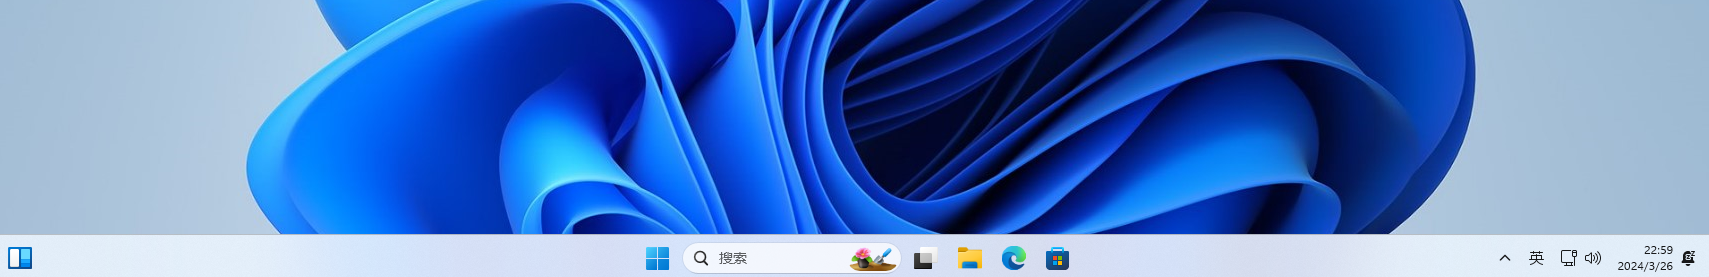
\includegraphics[width=.9\textwidth]{assets/advanced/taskbar.png}
  \caption{Windows 11 的默认任务栏样式}
  \label{fig:taskbar}
\end{figure}

如同 Windows 8 时候的操作一般,这一改动收获了不少批评。于是,微软迅速更新了能够调整这个设置的菜单。右键单击任务栏,点选【任务栏设置】,找到【任务栏行为】,点开它,第一项就是【任务栏对齐选项】的设置,将它改成靠左即可。

\section{使用旧版右键菜单}

Windows 11 在「文件资源管理器」(包括桌面)中引入了一套新的右键菜单,如\autoref{fig:Windows11_Right_click} 所示。

这套新的右键菜单虽然相比旧式菜单略显美观,但在很多时候并不实用:先不说这个新式菜单的 bug(例如「属性」之下的选项在第一次唤出菜单时不见了),由于今天的大多数应用仍然没有接入这套新的菜单系统,很多时候我们不得不在右键后点选【显示更多选项】这一项来打开旧式菜单以找到我们需要的功能。

大约在 2022 年 9 月末,微软发布了 Windows 11 版本 22H2 更新,新功能之一便是:在按住 \keys{Shift} 时点击右键,就能直接唤出旧式右键菜单。这显然比之前方便不少,但还是有些捉襟见肘。因此,在新式菜单完全成熟之前,我们可以通过下面的方法来始终使用旧式菜单。

\begin{figure}[htb!]
  \centering
  \begin{minipage}{.45\textwidth}
    \centering
    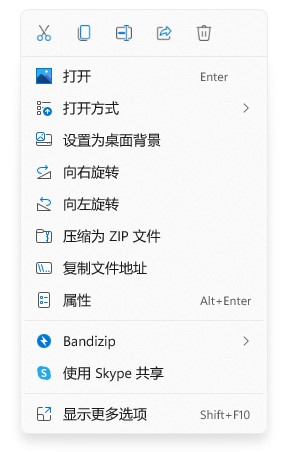
\includegraphics[width=.9\textwidth]{assets/advanced/Windows11_Right_click.jpg}
    \caption{Windows 11 的新式右键菜单}
    \label{fig:Windows11_Right_click}
  \end{minipage}
  \begin{minipage}{.54\textwidth}
    \centering
    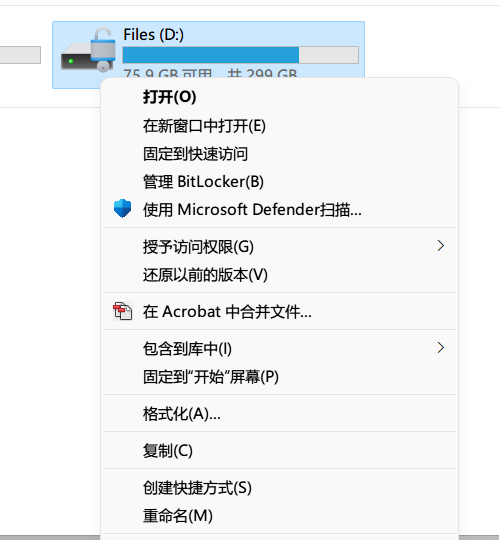
\includegraphics[width=.9\textwidth]{assets/advanced/Old_right_click.png}
    \caption{操作之后,将换回原来的旧式右键菜单}
    \label{fig:Old_right_click}
  \end{minipage}
\end{figure}

设置的方法如下:

\begin{itemize}
  \item 按 \keys{\Windows + X},选择【终端管理员】,然后选择【是】。(旧称「Windows Powershell(管理员)」或「Windows 终端(管理员)」。)
  \item 输入这行命令,然后按一次回车。重启后即见效果。
    \begin{MissingVerbatim}
      reg add "HKCU\Software\Classes\CLSID\{86ca1aa0-34aa-4e8b-a509-50c905bae2a2}\InprocServer32" /f /ve
    \end{MissingVerbatim}
\end{itemize}

这样设置之后,在文件资源管理器(包括桌面)中右键,都将继续使用旧式菜单,如\autoref{fig:Old_right_click} 所示。

如果需要返回新版菜单,使用下面这行命令:

\begin{MissingVerbatim}
  reg delete "HKCU\Software\Classes\CLSID\{86ca1aa0-34aa-4e8b-a509-50c905bae2a2}" /f
\end{MissingVerbatim}

\section{使用旧版资源管理器}

在 Windows 11 21H2 版本更新后,资源管理器变成了这样:

\begin{figure}[htb!]
  \centering
  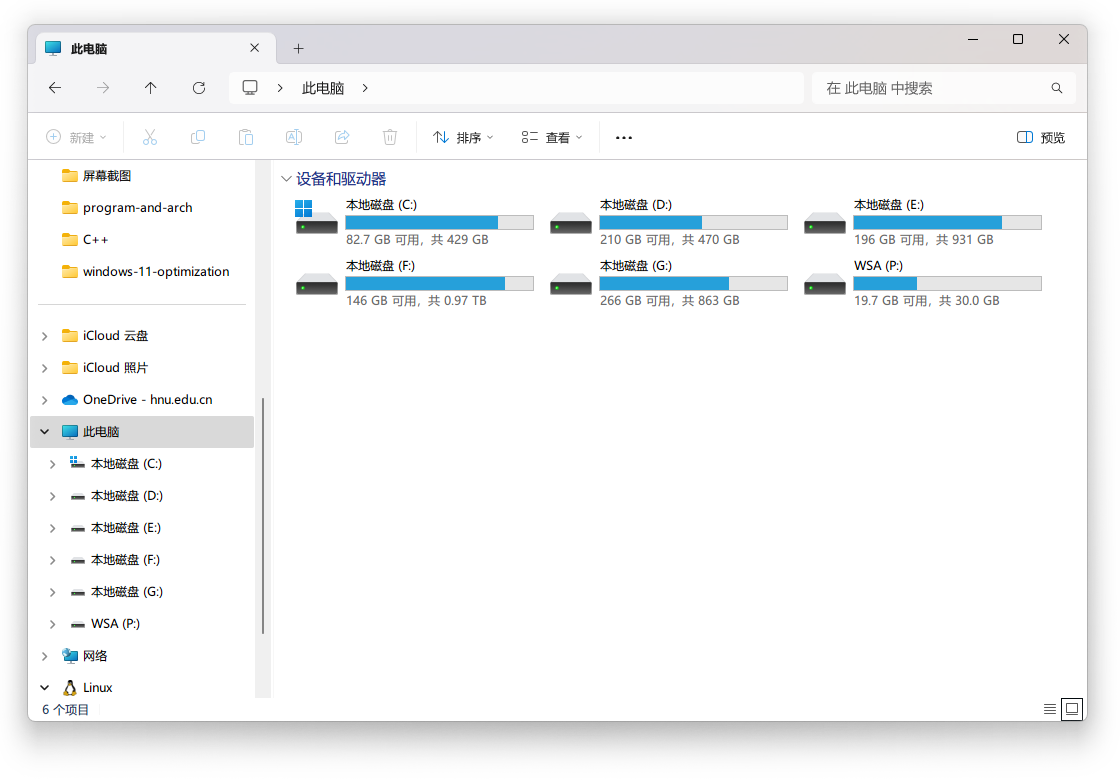
\includegraphics[width=.65\textwidth]{assets/advanced/new-explorer.png}
  \caption{Windows 11 的新资源管理器}
  \label{fig:new-explorer}
\end{figure}

曾经上方便捷的大按钮(或称「Ribbon 菜单」)已无影无踪,转而以 Windows 11 样式呈现。对已经习惯,甚至依赖旧式菜单那方便快捷操作的用户来说,这无疑是雪上加霜。不过,按照 Windows 一贯的兼容性,旧版资源管理器一定还在系统中。的确,不仅如此,甚至还有多种办法调出它。

\subsection{临时调出旧版资源管理器}

临时调出旧版资源管理器的方法有一种类似「曲线救国」的感觉:

\begin{itemize}
  \item 打开资源管理器,点击地址栏第一个向右的箭头,选择【控制面板】;
  \item 再如法炮制,这次选择【此电脑】;
    \begin{figure}[htb!]
      \begin{minipage}{.49\textwidth}
        \centering
        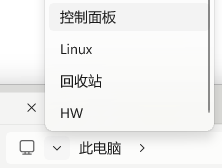
\includegraphics[width=.6\textwidth]{assets/advanced/go-to-control.png}
        \caption{先点选【控制面板】}
        \label{fig:go-to-control}
      \end{minipage}
      \begin{minipage}{.49\textwidth}
        \centering
        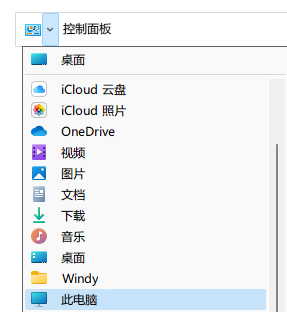
\includegraphics[width=.6\textwidth]{assets/advanced/back-to-this-pc.png}
        \caption{再点击【此电脑】}
        \label{fig:back-to-this-pc}
      \end{minipage}
    \end{figure}
  \item 成了。
    \begin{figure}[htb!]
      \centering
      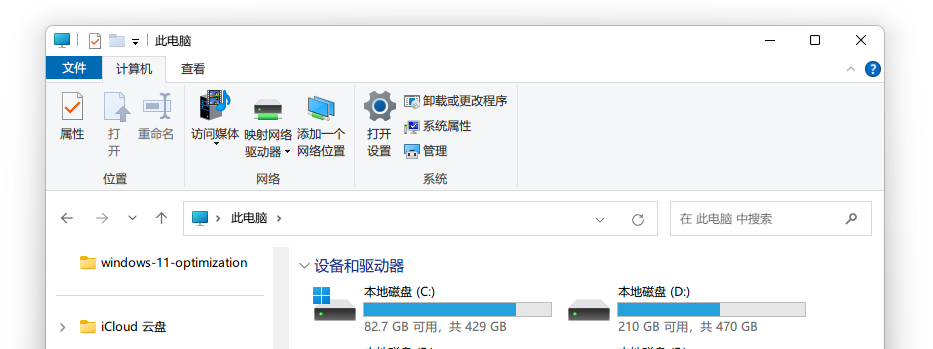
\includegraphics[width=.65\textwidth]{assets/advanced/old-explorer.png}
      \caption{恭喜你成功回到旧版资源管理器}
      \label{fig:old-explorer}
    \end{figure}
\end{itemize}

\subsection{永久使用旧版资源管理器}

不同于使用旧版右键菜单,永久切换旧版资源管理器的操作复杂一些。转到系统设置→【系统】→【系统信息】,查看「Windows 规格」下的「版本」,不同的系统版本需要采用不同的操作。

\subsubsection{21H2}

若版本是 21H2,操作就像上文的「使用旧版右键菜单」一样,只是把执行的命令换成以下这行,重启即可见效。

\begin{MissingVerbatim}
  reg add "HKLM\SOFTWARE\Microsoft\Windows\CurrentVersion\Shell Extensions\Blocked" /f /v "{e2bf9676-5f8f-435c-97eb-11607a5bedf7}"
\end{MissingVerbatim}

如果想恢复新版资源管理器,执行下面这行命令,依然是重启见效。

\begin{MissingVerbatim}
  reg delete "HKLM\SOFTWARE\Microsoft\Windows\CurrentVersion\Shell Extensions\Blocked" /f /v "{e2bf9676-5f8f-435c-97eb-11607a5bedf7}"
\end{MissingVerbatim}

\subsubsection{22H2 及以上}

适用于 22H2 及以上版本系统的方法不太一样:

\begin{itemize}
  \item 找一个你喜欢的地方,新建一个文件,命名为 \MissingTT{ribbon.reg} (注意,此文件的扩展名是 \MissingTT{reg},记得预先将「显示文件扩展名」打开);
  \item 用记事本打开刚刚的文件,写入以下内容,保存:
    \begin{MissingVerbatim}
Windows Registry Editor Version 5.00

[HKEY_CURRENT_USER\Software\Classes\CLSID\{2aa9162e-c906-4dd9-ad0b-3d24a8eef5a0}]
@="CLSID_ItemsViewAdapter"

[HKEY_CURRENT_USER\Software\Classes\CLSID\{2aa9162e-c906-4dd9-ad0b-3d24a8eef5a0}\InProcServer32]
@="C:\\Windows\\System32\\Windows.UI.FileExplorer.dll_"
"ThreadingModel"="Apartment"

[HKEY_CURRENT_USER\Software\Classes\CLSID\{6480100b-5a83-4d1e-9f69-8ae5a88e9a33}]
@="File Explorer Xaml Island View Adapter"

[HKEY_CURRENT_USER\Software\Classes\CLSID\{6480100b-5a83-4d1e-9f69-8ae5a88e9a33}\InProcServer32]
@="C:\\Windows\\System32\\Windows.UI.FileExplorer.dll_"
"ThreadingModel"="Apartment"
    \end{MissingVerbatim}
  \item 关掉记事本,双击 \MissingTT{ribbon.reg},点两下【是】,点【确定】;
  \item 用任务管理器重启文件资源管理器即可见效。
\end{itemize}

如果想回到新版的资源管理器,需要与之差不多的操作:

\begin{itemize}
  \item 找一个你喜欢的地方,新建一个文件,命名为 \MissingTT{restore.reg} (注意,此文件的扩展名是 \MissingTT{reg},记得预先将「显示文件扩展名」打开);
  \item 用记事本打开刚刚的文件,写入以下内容,保存:
    \begin{MissingVerbatim}
Windows Registry Editor Version 5.00

[-HKEY_CURRENT_USER\Software\Classes\CLSID\{2aa9162e-c906-4dd9-ad0b-3d24a8eef5a0}]

[-HKEY_CURRENT_USER\Software\Classes\CLSID\{6480100b-5a83-4d1e-9f69-8ae5a88e9a33}]
    \end{MissingVerbatim}
  \item 关掉记事本,双击 \MissingTT{restore.reg},点两下【是】,点【确定】;
  \item 用任务管理器重启文件资源管理器即可见效。
\end{itemize}

这两个文件可以一直留着,以备不时之需。

此外,若不喜欢繁琐的操作,更简单的方法是求助于第三方软件,例如 ExplorerPatcher。ExplorerPatcher 也附带了其他「回退到旧版」的功能,例如右键菜单或任务栏等,我们在\chapref{cha:tools-software} 中已有介绍。

\section{禁止资源管理器中的 \keys{F1} 打开 Edge 浏览器搜索帮助}

在 Windows 10 和 Windows 11 中,在「资源管理器」中按下 \keys{F1} 键,会自动调用 Edge 浏览器并打开一个必应搜索帮助的页面。该功能不随用户修改默认浏览器而改变,而搜索出来的帮助内容则完全没有帮助作用:

\begin{figure}[htb!]
  \centering
  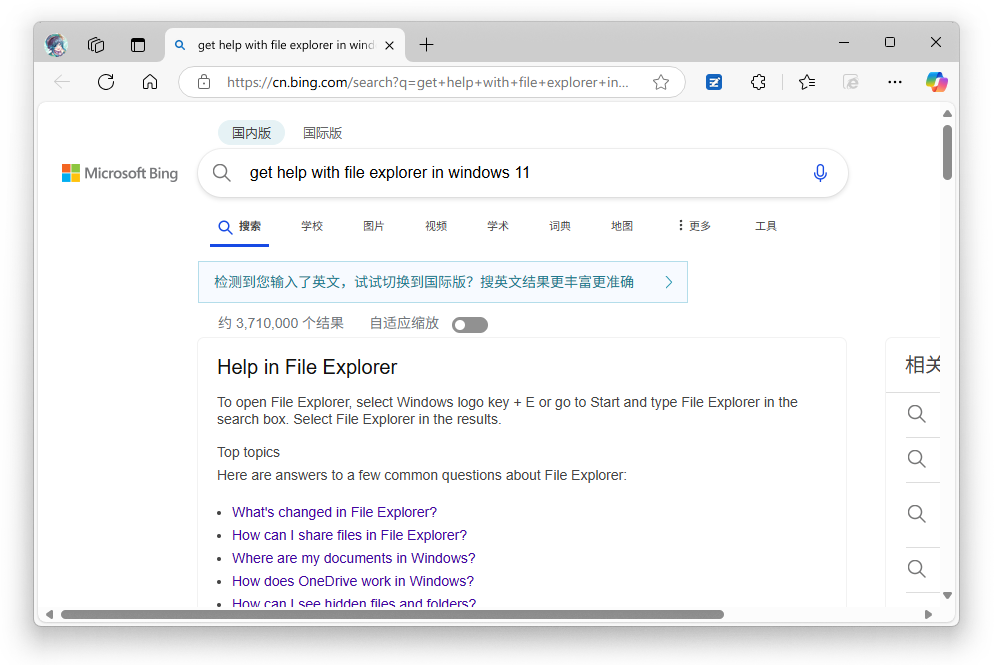
\includegraphics[width=.7\textwidth]{assets/advanced/F1_help_browser.png}
  \caption{没用的帮助}
  \label{fig:F1_help_browser}
\end{figure}

可以通过如下的方式,禁用这一行为。此方法在 Windows 10 中亦可使用。

\begin{itemize}
  \item 找一个你喜欢的地方,新建一个文件,命名为 \MissingVerb{disable_f1_help_in_explorer.reg} (注意,此文件的扩展名是 \MissingTT{reg},记得预先将「显示文件扩展名」打开);
  \item 用记事本打开刚刚的文件,写入以下内容,保存:
    \begin{MissingVerbatim}
Windows Registry Editor Version 5.00

[HKEY_CURRENT_USER\SOFTWARE\Classes\Typelib\{8cec5860-07a1-11d9-b15e-000d56bfe6ee}\1.0\0\win32]
@=""

[HKEY_CURRENT_USER\SOFTWARE\Classes\Typelib\{8cec5860-07a1-11d9-b15e-000d56bfe6ee}\1.0\0\win64]
@=""
    \end{MissingVerbatim}
  \item 关掉记事本,双击刚才编辑的文件,点两下【是】,点【确定】;
  \item 此时在资源管理器中按 F1 键,就不会再打开 Edge 浏览器了。
\end{itemize}

如果想恢复该功能,则使用如下的内容:

\begin{MissingVerbatim}
Windows Registry Editor Version 5.00

[-HKEY_CURRENT_USER\SOFTWARE\Classes\Typelib\{8cec5860-07a1-11d9-b15e-000d56bfe6ee}\1.0\0]
\end{MissingVerbatim}

你可以将这两个 \MissingTT{reg} 文件留着,以备不时之需。

\practice

如果你不习惯 Windows 11 的某些改变,不妨按本章提供的方法进行修整。
